\documentclass[11pt,a4paper]{article}
% The maths package
\usepackage{amsmath,mathtools,braket,amssymb, amsfonts}
\usepackage{fullpage}
\usepackage{graphicx}
\usepackage{tikz}
\usepackage[procnames]{listings}
\usepackage{color}

% New commands
\newcommand*\tageq{\refstepcounter{equation}\tag{\theequation}}
\newcommand*\circled[1]{\tikz[baseline=(char.base)]{
            \node[shape=circle,draw,inner sep=2pt] (char) {#1};}}

\begin{document}

% Colouring of Python Code
\definecolor{keywords}{RGB}{255,0,90}
\definecolor{comments}{RGB}{0,0,113}
\definecolor{red}{RGB}{160,0,0}
\definecolor{green}{RGB}{0,150,0}
 
\lstset{language=Python, 
        basicstyle=\ttfamily\small, 
        keywordstyle=\color{keywords},
        commentstyle=\color{comments},
        stringstyle=\color{red},
        showstringspaces=false,
        identifierstyle=\color{green},
        procnamekeys={def,class}}


\begin{titlepage}
\renewcommand{\baselinestretch}{1.0}
\begin{center}

\vspace*{30mm}
\Huge\bf
		Analysis of Steady State Flow in Systems\\
\vspace{20mm}
\large\sl
		by\\
		Ryan Mitchell
		\medskip\\
\rm
\large\sl
		for\\
		MECH2700\\
		Numerical Analysis I\\
\vspace{25mm}
		19 Oct 2015.		
\end{center}
\end{titlepage}


\tableofcontents
\listoffigures
%\listoftables
\newpage

\section{Introduction}

Most systems display attributes of both a transient and steady state response. A transient response, also known as the warm up period, is the initial flow that moves through the network and charges / fills storage devices. The network has to be able to contain these surges and influxes without breaking. As the system reaches an equilibrium condition, also known as the steady state, it becomes easier and more predictable to model.\\

Once the system has reached steady state the system can be analysed analytically in a number of ways. Simple systems can be analysed by hand but as the complexity of the system grows the time requirement for hand calculations increases dramatically. If a steady state system can be described in the form of a set of constraints on all the unknown flow quantities, and the vector of values satisfies all the equations simultaneously, a computer can be used to decrease computational time. If the simultaneous equations can be modelled as a matrix, the processing time is further reduced.\\

This assignment looks at two network systems and the methods behind solving them:

\begin{enumerate}
  \item A Chebyshev Filter
  \item A Water-Supply Network
\end{enumerate}

A Chebyshev Filter is a high-order filter excellent performance. It is built with passive components and filters electrical signals. The filter contains a system of linear constraint equations but the coefficients as well as the unknown values can be complex numbers. The Water-Supply Network is a network of pipes with the flow of water being described / given. The network contains a system of non-linear constraint equations but the coefficients are real numbers.\\

\bigskip
This assignment makes use of the Gauss-Jordan matrix elimination method. This method uses row-reduction to  modify the values of the lower left-hand corner of the matrix until it is filled with zeros. Once complete the matrix is said to be an upper triangular matrix in row echelon form. Once all the leading non-zero entries on the diagonal are reduced to 1 the matrix is a reduced row echelon matrix. There are three types of elementary row operations:
\begin{enumerate}
  \item Swapping two rows,
  \item Multiplying a row by a non-zero number
  \item Adding a multiple of one row to another row
\end{enumerate}
This solver has been designed to handle floats and complex numbers and the code can be seen in Section \ref{sec:GaussJordanCode}. 

\newpage

\section{General Gauss-Jordan Function} \label{sec:GaussJordanCode}
\lstinputlisting[language=Python]{gjSolver.py}
\newpage

\section{A Chebyshev Filter For Electrical Signals} \label{sec:Cheb}

\medskip	
\begin{figure}[h]
	\centering
	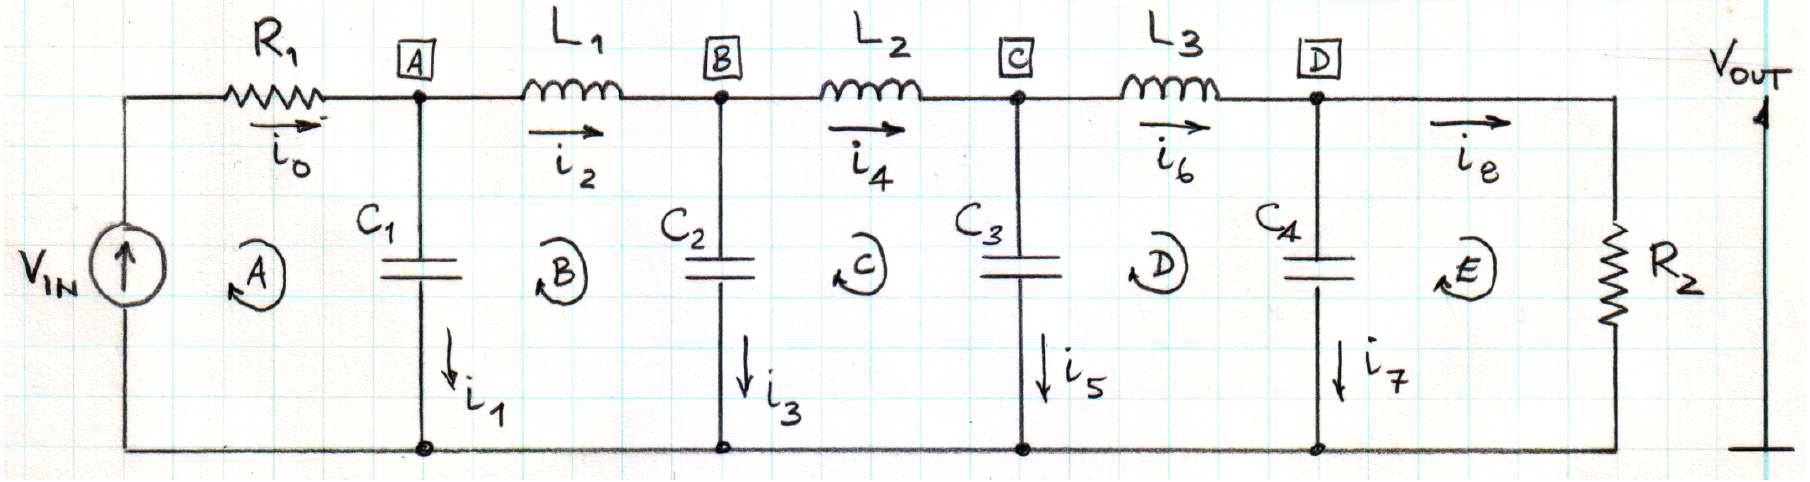
\includegraphics[width=0.9\linewidth]{Images/Circuit.png}
	\caption{Chebyshev Filter Circuit}
	\label{fig:circuit}
\end{figure}

To analyse the circuit provided in Figure \ref{fig:circuit}, Mesh and Nodal Analysis techniques are used. Mesh Analysis is derived from Kirchoff's Voltage Law which states that `the directed sum of the electrical potential differences (voltage) around any closed network is zero'. Nodal Analysis is derived form Kirchoff's Current Law which states that `at any node (junction) in an electrical circuit, the sum of currents flowing into that node is equal to the sum of currents flowing out of that node'. Both tools are required to derive the nine equations in order to solve for the unknowns, $\omega$ and $V_{IN}$, in the system. The five Mesh equations (equations \ref{eq:1} to \ref{eq:5}) and four Node equations (equations \ref{eq:6} to \ref{eq:9}) were found to be

\begin{align}
	&\circled{A} \quad V_{IN} - Z_{R1}i_{0} - Z_{C1}i_{1} = 0 \tageq\label{eq:1}\\
	&\quad \quad \, \, V_{IN} = Z_{R1}i_{0} + Z_{C1}i_{1} \notag \\
	&\circled{B} \quad Z_{C1}i_{1} - Z_{L1}i_{2} - Z_{C2}i_{3} = 0 \tageq\label{eq:2}\\
	&\circled{C} \quad Z_{C2}i_{3} - Z_{L2}i_{4} - Z_{C3}i_{5} = 0 \tageq\label{eq:3}\\
	&\circled{D} \quad Z_{C3}i_{5} - Z_{L3}i_{6} - Z_{C4}i_{7} = 0 \tageq\label{eq:4}\\
	&\circled{E} \quad Z_{C4}i_{7} - Z_{R2}i_{8} = 0 \tageq\label{eq:5}
\end{align}
\begin{align}
	&\boxed{A} \quad i_{0} - i_{1} - i_{2} = 0 \tageq\label{eq:6}\\
	&\boxed{B} \quad i_{2} - i_{3} - i_{4} = 0 \tageq\label{eq:7}\\
	&\boxed{C} \quad i_{4} - i_{5} - i_{6} = 0 \tageq\label{eq:8}\\
	&\boxed{D} \quad i_{6} - i_{7} - i_{8} = 0 \tageq\label{eq:9}
\end{align}\\

These equations can then be compiled into matrix form in order to make use of software tools.\\

$\begin{bmatrix*}
	Z_{R1} & Z_{C1} & 0 & 0 & 0 & 0 & 0 & 0 & 0 \\
	0 & Z_{C1} & -Z_{L1} & -Z_{C2} & 0 & 0 & 0 & 0 & 0\\
	0 & 0 &  0 & Z_{C2} & -Z_{L2} & -Z_{C3} & 0 & 0 & 0\\
	0 & 0 & 0 & 0 & 0 & Z_{C3} & -Z_{L3} & -Z_{C4} & 0\\
	0 & 0 & 0 & 0 & 0 & 0 & 0 & Z_{C4} & -Z_{R2}\\
	1 & -1 & -1 & 0 & 0 & 0 & 0 & 0 & 0\\
	0 & 0 & 1 & -1 & -1 & 0 & 0 & 0 & 0\\
	0 & 0 & 0 & 0 & 1 & -1 & -1 & 0 & 0\\
	0 & 0 & 0 & 0 & 0 & 0 & 1 & -1 & -1\\
\end{bmatrix*}$
$ * $
$\begin{bmatrix}
	i_{0}\\
	i_{1}\\
	i_{2}\\
	i_{3}\\
	i_{4}\\
	i_{5}\\
	i_{6}\\
	i_{7}\\
	i_{8}\\
\end{bmatrix}$
$ = $
$\begin{bmatrix}
	V_{IN}\\
	0\\
	0\\
	0\\
	0\\
	0\\
	0\\
	0\\
	0\\
\end{bmatrix}$ \bigskip

Which becomes \\

$\begin{bmatrix*}
	R_{1} & \frac{-j}{\omega C_{1}} & 0 & 0 & 0 & 0 & 0 & 0 & 0 \\
	0 & \frac{-j}{\omega C_{1}} & -j \omega L_{1} & \frac{j}{\omega C_{2}} & 0 & 0 & 0 & 0 & 0\\
	0 & 0 &  0 & \frac{-j}{\omega C_{2}} & -j \omega L_{2} & \frac{j}{\omega C_{3}} & 0 & 0 & 0\\
	0 & 0 & 0 & 0 & 0 & \frac{-j}{\omega C_{3}} & -j \omega L_{3} & \frac{j}{\omega C_{4}} & 0\\
	0 & 0 & 0 & 0 & 0 & 0 & 0 & \frac{-j}{\omega C_{4}} & -R_{2}\\
	1 & -1 & -1 & 0 & 0 & 0 & 0 & 0 & 0\\
	0 & 0 & 1 & -1 & -1 & 0 & 0 & 0 & 0\\
	0 & 0 & 0 & 0 & 1 & -1 & -1 & 0 & 0\\
	0 & 0 & 0 & 0 & 0 & 0 & 1 & -1 & -1\\
\end{bmatrix*}$
$ * $
$\begin{bmatrix}
	i_{0}\\
	i_{1}\\
	i_{2}\\
	i_{3}\\
	i_{4}\\
	i_{5}\\
	i_{6}\\
	i_{7}\\
	i_{8}\\
\end{bmatrix}$ 
$ = $
$\begin{bmatrix}
	V_{IN}\\
	0\\
	0\\
	0\\
	0\\
	0\\
	0\\
	0\\
	0\\
\end{bmatrix}$

Need to check for singularity of the matrix as the first step of the function!

\subsection{Conclusion}

\newpage

\section{A Water-Supply Network} \label{sec:pipes}

\medskip
\begin{figure}[h]
	\centering	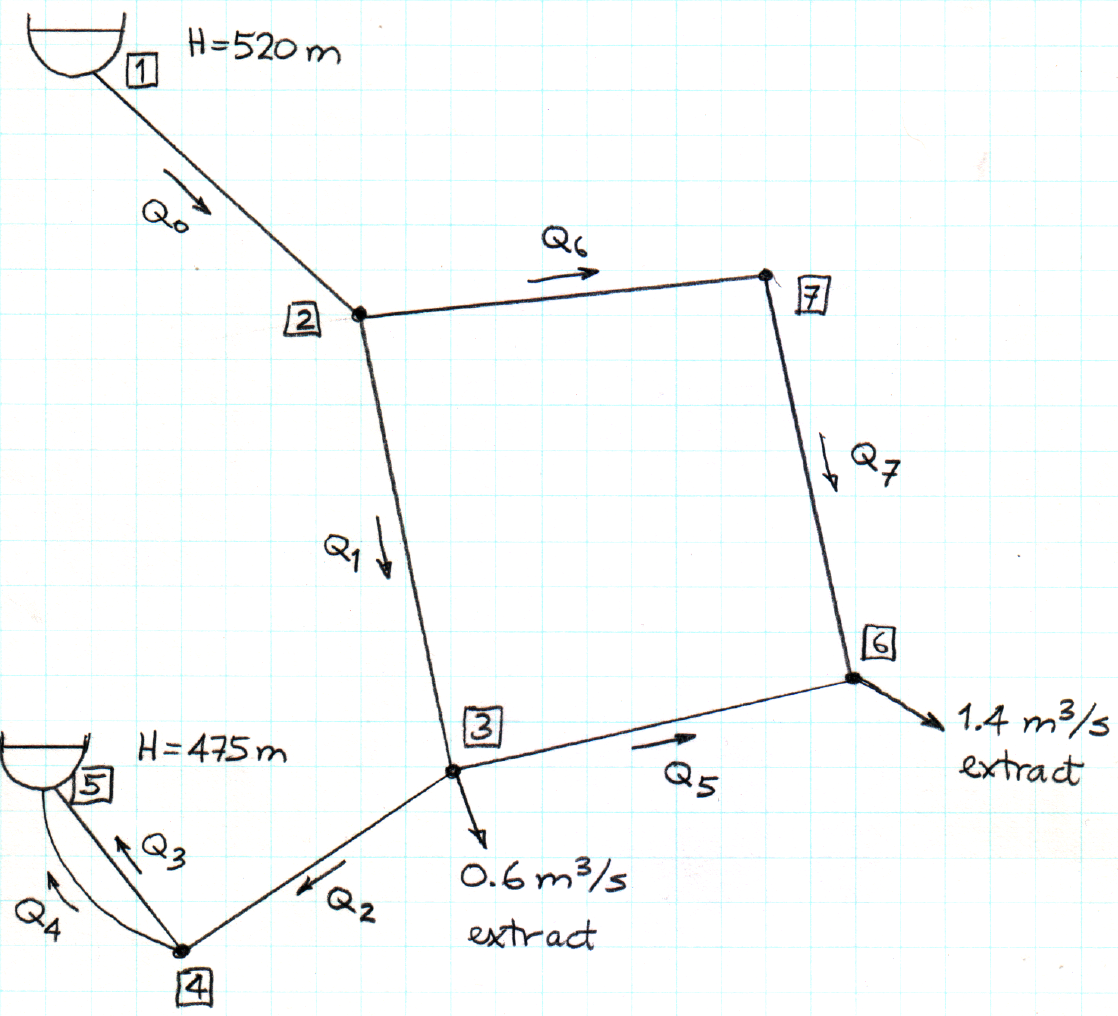
\includegraphics[width=0.6\linewidth]{Images/PipeNetwork.png}
	\caption{A Water-Supply Network}
	\label{fig:PipeNetwork}
\end{figure}

\subsection{Conclusion}

\end{document}
